\chapter{流匹配、Rectified Flow、最优运输与桥问题}
\label{th:flow}

\section{从可采样的条件路径到不可求的边缘速度}

给定辅助变量 $Z$（例如一对端点），假设条件密度与速度满足
$\partial_t p_t(x\mid Z)+\nabla\cdot(p_t(x\mid Z)u_t(x\mid Z))=0$。
对 $Z$ 积分，定义
\begin{equation}\label{th:fm-marginal}
p_t(x)=\E_Zp_t(x\mid Z),\qquad
u_t(x)=\E[u_t(x\mid Z)\mid X_t=x].
\end{equation}
则 $p_tu_t=\E_Z[p_t(x\mid Z)u_t(x\mid Z)]$，因此边缘也满足连续性方程。
这是一个概率通量恒等式，不只是模型经验。条件路径若是确定性插值、
条件分布为 Dirac 测度，可在相应可积条件下用连续性方程的弱形式表述。

可训练的条件流匹配损失为
\begin{equation}\label{th:cfm}
\mathcal L_{\rm CFM}=\E_{t,Z,X_t\mid Z}
 w(t)\|u_\theta(X_t,t)-u_t(X_t\mid Z)\|^2.
\end{equation}
按式\eqref{th:conditional-mean}，它与边缘流匹配只差不含预测函数的项。
训练可以完全不求解 ODE，因此常称 simulation-free；
生成仍通常需要沿学到的边缘速度求解 ODE。

\section{线性插值与方向约定}

取端点耦合 $\gamma(x_0,\epsilon)$，边缘分别是数据与标准高斯，构造
\[
X_t=(1-t)X_0+t\epsilon,\qquad U^{\rm cond}=\epsilon-X_0.
\]
最简单是独立耦合 $\gamma=p_0\otimes\mathcal N(0,I)$。
训练采样均匀 $t$ 或指定的时间密度，回归条件位移。
推理从1走向0，更新为 $x_{t+h}=x_t+h u_\theta(x_t,t)$，$h<0$。
某些教程从噪声0走向数据1，标签则为 $x_{\rm data}-x_{\rm noise}$；
换约定要同时换时间、标签与更新方向。

条件路径可使用非零方差高斯管道，也可用一般随机插值
$I_t(X_0,X_1)+\gamma_t\eta$。
端点、噪声系数与可微性决定它满足什么边缘方程；
“stochastic interpolant”不等于任意加噪就自动获得正确逆 SDE。

\section{为什么直线标签不保证一步生成}

对固定端点，一条条件轨迹的速度恒定。
但多个端点对可能经过同一位置，网络只能看到 $(x,t)$，
学习到的是这些方向的后验平均。积分边缘速度形成的轨迹可以弯曲。
因此一步 Euler 误差与 $\partial_tu+Du\,u$ 有关，
并不因为每个训练标签是端点位移就必然为零。

一个显式例子是 $X_0\sim\mathcal N(0,1)$ 与 $\epsilon\sim\mathcal N(0,1)$ 独立。
此时路径方差 $c_t=(1-t)^2+t^2$，
\[
u_t(x)=\frac{2t-1}{c_t}x.
\]
两端分布相同，而中间方差先收缩后扩张，速度并非恒定。
在 $t=1$，$u_1(x)=x$；一步反向 Euler 会给出 $x_0=x_1-u_1(x_1)=0$，
错误地压成一个点。精确 ODE 积分的端点分布却仍是标准高斯。

\begin{figure}[htbp]
\centering
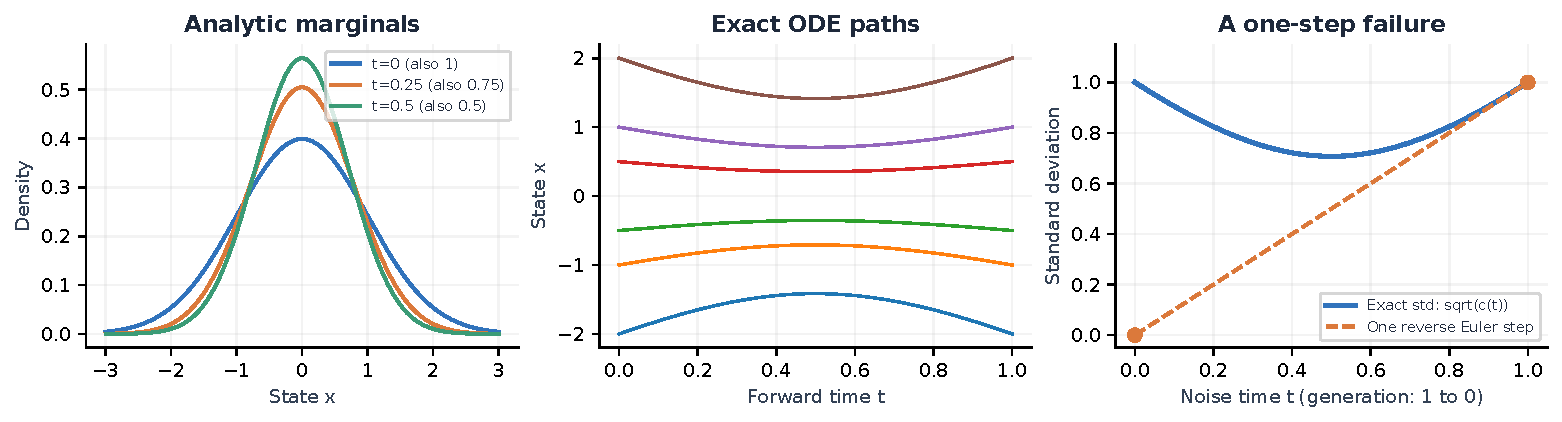
\includegraphics[width=\linewidth]{assets/theory/gaussian-path.pdf}
\caption{独立高斯端点的线性插值。左图为解析密度，中图为准确 ODE 轨迹，
右图为初始标准差1时的精确值与一步 Euler 结果。图为本书解析示例，不是模型实验。}
\end{figure}

\section{Reflow 改变耦合，而不是证明最优}

Rectified Flow 可先学习一个运输 ODE，
再用它把噪声与生成结果配对，在新配对上训练直线路径。
重新配对使监督更贴近既有生成轨迹，常用于降低曲率与改善少步采样。
它需要生成配对数据与额外训练，不能把 reflow 解释成无成本换 scheduler。

在理想场和特定凸成本等假设下可讨论直化与成本性质，
但有限容量、数值误差与训练数据分布都会影响结果。
不能无条件宣称任何 reflow 迭代都严格达到二次成本最优映射，
也不能把一个模型在某分辨率的一步结果推广到所有条件任务。

\section{静态 OT、动态 OT 与概率流的区别}

二次 Kantorovich 问题为
\[
\inf_{\gamma\in\Pi(p_0,p_1)}\E_\gamma\|X_1-X_0\|^2.
\]
Monge 问题限制为确定映射 $X_1=T(X_0)$，需要额外存在性条件。
Benamou--Brenier 动态形式在合适条件下等价：
\begin{equation}\label{th:bb-ot}
\inf_{p_t,u_t}\int_0^1\int p_t(x)\|u_t(x)\|^2\mathrm dx\mathrm dt,
\quad \partial_tp_t+\nabla\cdot(p_tu_t)=0,
\end{equation}
并固定两端分布。它同时优化整条密度路径与速度。
普通扩散通常预先选定高斯扰动路径，不是在这些路径中优化动作量。
即便每一刻分数是梯度场，复合后的端点映射也不自动是 OT 最优映射。

小批次 OT 配对用于选择训练耦合。
有限 batch 的最优配对与总体分布的最优耦合有统计差异，
熵正则 Sinkhorn 解还优化了带正则项的不同问题。
所谓“OT path”必须说明是条件端点间的直线，还是总体分布的位移插值。

\section{Schrödinger Bridge 与已知扩散的时间反演}

Schrödinger Bridge 给定参考随机过程 $R$，在端点边缘受约束的路径测度中求
\[
\inf_{P:\,P_0=p_0,\ P_T=p_1}\KL(P\Vert R).
\]
它优化的是相对于参考过程的随机路径；小噪声极限与 OT 的联系需要专门条件。
Score SDE 时间反演则从一个已选的正向加噪过程出发，恢复它的逆过程。
如果参考过程、端点和控制问题被特殊选择，二者可以联系；
一般情况下，反向扩散不自动解决任意给定两端的桥问题。

\Needspace{17\baselineskip}
\section{速度场并不由边缘分布唯一决定}

若 $u$ 满足连续性方程，而 $w$ 满足 $\nabla\cdot(p_tw)=0$，
则 $u+w$ 产生相同密度演化。
边缘约束允许额外的无散概率环流。
不同条件耦合、动力学成本与正则条件可以选择不同速度场，
所以“所有方法具有相同的边缘”仍不足以断言其轨迹相同。

\begin{theorytakeaway}
流匹配的核心是条件通量平均。直线路径、总体 OT、桥问题和一步生成是四个不同层次。
它们可以联系，但每一步都要补充耦合、成本、正则性或训练条件。
\end{theorytakeaway}
\threading{主参考第5--7章\cite{theorybook}；条件流匹配、Rectified Flow 与实现约定见
\cite{fm,rf,flow-guide}。本章给出一个可解析的反例，解释“直线监督不等于一步精确生成”。}
